% !TeX root = ../../latex-talk.tex

\part{SJTUBeamer}

\begin{frame}
  \frametitle{简介}
  \begin{columns}
    \begin{column}{0.6\textwidth}
      \begin{itemize}
        \item 最早由谌翔于 2021 年 4 月发布
        \item 2021 年 5 月起由 SJTUG 接手,发布 1.0 版
        \item 2021 年 9 月李子龙重构了整个宏包的代码,升级版本号为 2.0
        \item 最新版:\SJTUBeamerVersion{} (\SJTUBeamerDate)
        \item 支持三种基本样式与扩展样式的幻灯片模板
        \item 支持镜像站克隆 \link{https://mirror.sjtu.edu.cn/git/SJTUBeamer.git/},支持使用任一引擎编译
      \end{itemize}
    \end{column}
    \begin{column}{0.4\textwidth}
      \begin{exampleblock}{}
        \begin{minipage}[c]{1cm}
          \includegraphics[width=0.8cm]{\getcontribpath{sjtug}{vi/sjtug}}
        \end{minipage}
        \begin{minipage}[c]{2cm}
          \href{https://github.com/sjtug}{sjtug}/\href{https://github.com/sjtug/SJTUBeamer}{SJTUBeamer}
        \end{minipage}
      \end{exampleblock}
      \vspace{-8pt}
      \begin{block}{}
        \scriptsize
        上海交通大学 Beamer 模版 | Beamer template for Shanghai Jiao Tong University
      \end{block}
      \vspace{-8pt}
      \begin{alertblock}{}
        \scriptsize
        \begin{tabular}{cl}
          \faStar       & 231 \\
          \faEye        & 6   \\
          \faCodeBranch & 13  \\
        \end{tabular}
      \end{alertblock}
    \end{column}
  \end{columns}
\end{frame}

\begin{frame}
  \frametitle{\only<1>{为什么使用 beamer 制作幻灯片?}\only<2>{当然也有新兴替代物}}
  \begin{columns}[t]

    \only<2>{
      \begin{column}{0.25\textwidth}
        \begin{block}{\faMarkdown{} 代码翻译}
          \begin{itemize}
            \item[\faVuejs{}] Slidev \link{https://cn.sli.dev/}
            \item[\faJsSquare{}] Marp \link{https://marp.app/}
            \item[\faJs{}] AutoBeamer \link{https://github.com/LogCreative/AutoBeamer}
          \end{itemize}
        \end{block}
        \note[item]<2>{\textbf{Markdown} 当然也有新兴替代物,比如可以从 Markdown 代码转换为幻灯片的一些软件。基于 Vue 的 Slidev 可以快速地输出灵活布局的幻灯片,基于 TypeScript 的 Marp 可以作为 VS Code 的插件来实时预览 Markdown 幻灯片,还有我制作的转换 Markdown 文档为 beamer 代码的 AutoBeamer 也欢迎大家的试用。}
      \end{column}
    }

    \begin{column}{0.25\textwidth}
      \begin{block}{\LaTeX{} SJTUBeamer}
        \begin{itemize}
          \item[\faPlus] \LaTeX{} 原生
          \item[\faPlus] 规范的格式
          \item[\faMinus] 美术功能麻烦
        \end{itemize}
      \end{block}
      \note[item]<1>{\textbf{Beamer} 是 \LaTeX{} 原生的幻灯片类,可以输入专业的公式,其编程式的方法会促使用户规整幻灯片的布局,更为容易地产生正式而不失优雅的幻灯片。我们使用 \LaTeX{} 主要也是为了符合规范,对于很多不擅长排版的小伙伴有个这样的工具自动美化自己的作品是一件非常方便的事情。

        当然缺点也是存在的,就是美术功能的实现较为复杂,以及一些多媒体的支持可能需要使用链接的形式。}
    \end{column}

    \only<2>{
      \begin{column}{0.25\textwidth}
        \begin{exampleblock}{\faApple{} Keynote}
          \begin{itemize}
            \item[\faPlus] 友好的界面
            \item[\faPlus] 精致的动画
            \item[\faMinus] 缺少进阶功能
          \end{itemize}
        \end{exampleblock}
        \note[item]<2>{\textbf{Keynote} 是苹果独占的幻灯片软件,相比于 PowerPoint 有了更加用户友好的界面,辅以一些精致的动画,可以较快地做出“果味”幻灯片。

          当然简单也会带来进阶功能的缺失,缺乏插件体系的支持,能做出的东西相比于 PowerPoint 少了不少。}
      \end{column}
    }

    \begin{column}{0.25\textwidth}
      \begin{exampleblock}{\faFilePowerpoint{} PowerPoint}
        \begin{itemize}
          \item[\faPlus] 灵活的插件
          \item[\faPlus] 强大的动画
          \item[\faMinus] 布局不够规整
        \end{itemize}
      \end{exampleblock}
      \note[item]<1>{\textbf{PowerPoint} 我们在前半部分的讲座中看到了 PowerPoint 制作幻灯片的强大之处,可见即可得,辅以强大的动画功能,并可以使用灵活的插件提高效率。

        当然灵活性也会让用户在布局上更加随意一些,并在这样一些细节上让整个演讲稿看起来慢慢地变得没有那么正式。当然你也可以只使用大纲视图编写幻灯片,来规整自己的布局。}
    \end{column}
  \end{columns}
\end{frame}

\begin{frame}
  \frametitle{浅学手册}

  \only<1>{
    \begin{columns}
      \begin{column}{0.7\textwidth}
        前往 SJTUBeamer 的发布页 \link{https://github.com/sjtug/SJTUBeamer/releases} 可以得到一个干净的 \pkg{sjtubeamer-ctan.zip},用于将该 SJTUBeamer 安装到本地目录。以及一些其他文档的下载。当然你也可以在 SJTUG 镜像站 \link{https://mirror.sjtu.edu.cn/} 上下载 SJTUBeamer 的这些 Assets。

        \begin{exampleblock}{\faGit* 从镜像站克隆最新版}
          \ttfamily\footnotesize
          git clone https://mirror.sjtu.edu.cn/git/SJTUThesis.git/
        \end{exampleblock}
      \end{column}
      \begin{column}{0.3\textwidth}
        \framebox{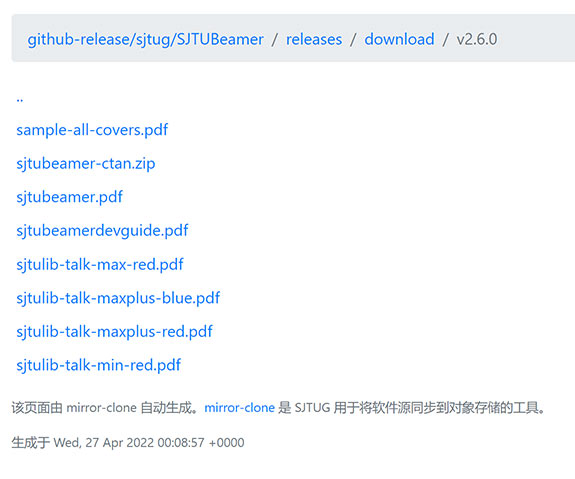
\includegraphics[width=\linewidth]{mirrorclone}}
      \end{column}
    \end{columns}
    \note{进入镜像站页面后,点击 git/SJTUBeamer.git。跳转可能稍有 BUG,所以可能要退回来再点一次即可进入该页面。}
  }

  \only<2>{
    \begin{columns}
      \begin{column}{0.7\textwidth}
        《SJTUBeamer 使用手册》\link{https://github.com/sjtug/SJTUBeamer/releases/download/v2.6.0/sjtubeamer.pdf} 给出了大量的示例,用于快速上手 SJTUBeamer 的基本使用方法。推荐大家从一个干净的文档一步步码出来这些例子,或者遇到问题先按手册查询。本讲座仅做概览。

        \begin{exampleblock}{\faTerminal{} 从源码编译文档}
          \ttfamily\footnotesize
          cd src\\
          \textcolor{gray}{\# 可以考虑缓存示例结果,在 l3build.lua 中修改 cachedemo=true} \\
          l3build doc
        \end{exampleblock}
      \end{column}
      \begin{column}{0.3\textwidth}
        \framebox{
\includegraphics[width=\linewidth]{sjtubeamerfirst}}
      \end{column}
    \end{columns}
  }

  \only<3>{
    \begin{columns}
      \begin{column}{0.7\textwidth}
        \textit{Development Guide of SJTUBeamer} \link{https://github.com/sjtug/SJTUBeamer/releases/download/v2.6.0/sjtubeamerdevguide.pdf} 对于想要了解 SJTUBeamer 框架与原理的人会比较有用,感兴趣的可以通过阅读该手册尝试对代码更改提 PR 或贡献插件 \link{https://github.com/sjtug/SJTUBeamer/issues/81}。本讲座不会涉及这一部分。
        \begin{exampleblock}{\faTerminal{} 代码同步}
          \ttfamily\footnotesize
          cd src\\
          \textcolor{gray}{\# 将 Doc\TeX{} 解包为 sty 文件并移至根目录} \\
          l3build check
        \end{exampleblock}
      \end{column}
      \begin{column}{0.3\textwidth}
        \framebox{
\includegraphics[width=\linewidth]{sjtubeamerdevguidefirst}}
      \end{column}
    \end{columns}
    \note{用英文写实际上是因为国内做 beamer 的比较少。sad。}
  }

\end{frame}

\begin{frame}[fragile]
  \frametitle{文档类设置}

  \only<1>{
    为文档类设置 \pkg{aspectratio} 选项可以更改幻灯片的长宽比。其他通用选项详见 \textit{The Beamer class -- User Guide} \link{https://mirrors.sjtug.sjtu.edu.cn/CTAN/macros/latex/contrib/beamer/doc/beameruserguide.pdf}。帧环境 \env{frame} 详见第 \ref{frame} 页。
  }

  \only<2>{
    SJTUBeamer 依赖于 \texttt{ctexbeamer} 文档类(如果编写英文幻灯片,可以直接使用 \texttt{beamer} 文档类),相关字体设置详见《\CTeX{} 宏集手册》\link{https://mirrors.sjtug.sjtu.edu.cn/CTAN/language/chinese/ctex/ctex.pdf}。
  }

  \begin{columns}
    \begin{column}{0.62\textwidth}
      \begin{codeblock}[]{\only<1>{更改长宽比}\only<2>{更改字体}}
|\highlightline|\documentclass[|\only<1>{aspectratio=169}\only<2>{fontset=fandol}|]{ctexbeamer}
\usetheme{sjtubeamer}
\begin{document}
  \begin{frame}
    \frametitle{||欢迎}
    ||你好,SJTUBeamer||!
||  \end{frame}
||\end{document}
      \end{codeblock}
    \end{column}
    \begin{column}{0.38\textwidth}
      \begin{center}
        \includebeamerlarge{welcome}
      \end{center}
    \end{column}
  \end{columns}
  
\end{frame}

\begin{frame}[fragile]
  \frametitle{切换设计}
  \begin{columns}
    \begin{column}{0.6\textwidth}

      \only<1>{
      为了使用 SJTUBeamer,需要在根目录中创建一个文件,并添加 \cmd{usetheme\{sjtubeamer\}}。你可以添加用逗号分隔的选项切换不同的设计样式。
      }

      \only<2>{
        还可以适配 \pkg{beamer} 自带的外样式,可以通过 \pkg{topright} 或 \pkg{bottomright} 选项切换徽标位置。
        \note{sidebar 外样式略有一些 BUG。}
      }

      \begin{codeblock}[]{}
\documentclass{ctexbeamer}
|\highlightline|\usetheme[|\only<1>{maxplus,blue,light}\only<2>{default,topright}|]{sjtubeamer}
\begin{document}
  \title{||使用 Beamer 制作学术报告幻灯片}
  \subtitle{||上海交通大学图书馆专题培训讲座}
  \author{||李子龙}
  \institute[SJTUG]{SJTU Linux User Group}
  \date{2022 年 5 月}
|\highlightline<1>|  \maketitle
|\highlightline<1>|  \part{||介绍}
|\highlightline<1>|  \makebottom
||\end{document}
      \end{codeblock}
    \end{column}
    \begin{column}{0.4\textwidth}
      \only<1>{
        \begin{figure}
          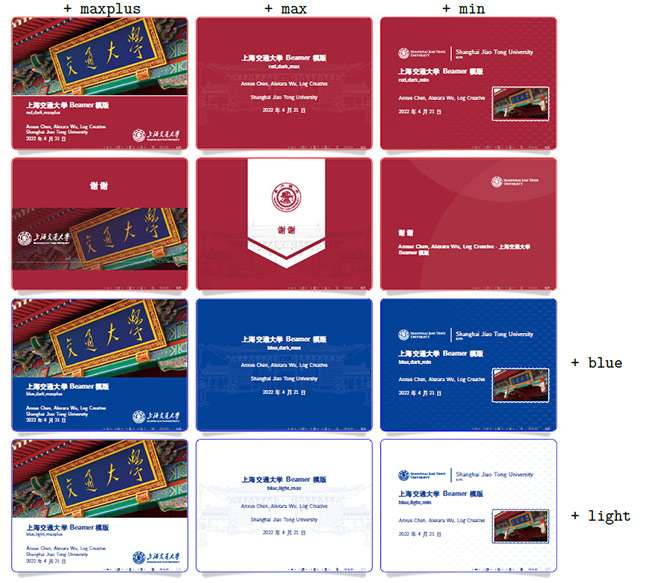
\includegraphics[width=\linewidth]{sjtubeamercover}
          \caption{封面样式}
        \end{figure}
      }
      \only<2>{
        \begin{figure}
          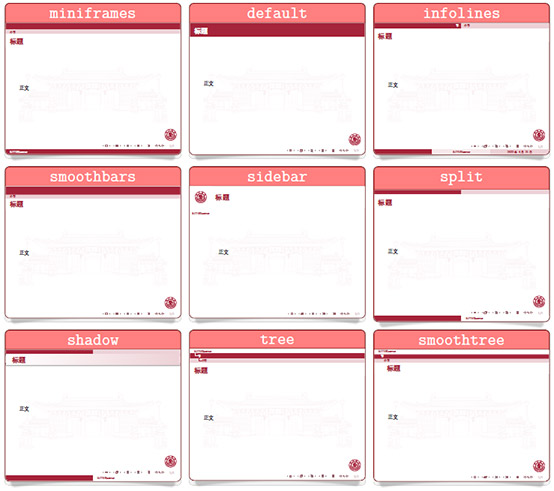
\includegraphics[width=\linewidth]{sjtubeamerouter}
          \caption{外样式}
        \end{figure}
      }
    \end{column}
  \end{columns}
\end{frame}


\begin{frame}
  \frametitle{符合交大视觉形象识别系统}

  \begin{table}
    \caption{上海交通大学视觉形象识别系统规范(节选)}
    \vspace*{-5pt}
    \begin{stampbox}
      \footnotesize
      \begin{tabular}{llll}
        \alert{编号}                                                   & \alert{说明}                   & \alert{编号}                                                   & \alert{说明}     \\
        \href{https://vi.sjtu.edu.cn/index.php/articles/base/1}{A1-06} & 校徽需 $\frac{1}{5}h$ 安全空间 & \href{https://vi.sjtu.edu.cn/index.php/articles/base/5}{A5-03} & 辅助图形使用规范 \\
        \href{https://vi.sjtu.edu.cn/index.php/articles/base/3}{A3-01} & 标准色规范(含色阶)           & \href{https://vi.sjtu.edu.cn/index.php/articles/base/5}{A5-05} & 辅助图形底纹制作 \\
        \href{https://vi.sjtu.edu.cn/index.php/articles/base/3}{A3-02} & 辅助色彩规范(含色阶)         & \href{https://vi.sjtu.edu.cn/index.php/articles/app/7}{B1-01}  & 名片             \\
        \href{https://vi.sjtu.edu.cn/index.php/articles/base/3}{A3-05} & 品牌专用色彩搭配表             & \href{https://vi.sjtu.edu.cn/index.php/articles/app/7}{B1-20}  & 文件封套         \\
        \href{https://vi.sjtu.edu.cn/index.php/articles/base/4}{A4-08} & 二级机构中英文名称横式组合     & \href{https://vi.sjtu.edu.cn/index.php/articles/app/8}{B2-02}  & PPT 模板         \\
      \end{tabular}
    \end{stampbox}
  \end{table}

  正如 SJTUThesis 需要依照学位论文规范一样,SJTUBeamer 借助于 \TikZ{} 实现了《上海交通大学视觉形象识别系统》\link{https://vi.sjtu.edu.cn/} 的绝大部分规范\footnote{使用规范所规定的用品需要遵守相关许可条例 \link{https://vi.sjtu.edu.cn/index.php/articles/bulletin/16}。}。

  \note[item]{我相信小米的二百万 logo 更改让大家意识到了视觉形象识别系统的存在。交大在 2016 年的时候颁布了自己的视觉形象识别系统,并配套了对应的 PPT 模板。}

  \note[item]{许可条例第十三条规定:“校属各单位及个人可以自行或委托其他单位制作《手册》中有明确范例的物品,须严格遵照《手册》的要求,不得自行改动”,\textsc{SJTUBeamer} 也就需要依照该规范制作产物。}
\end{frame}

\begin{frame}
  \frametitle{SJTU VI 对应的特殊方法}

  \begin{columns}
    \begin{column}{0.7\textwidth}

      \stamptext[sjtuRedPrimary]{注} \cmd{stamptext} 用于创建一个印记形状文本框。

      \begin{stampbox}[sjtuRedPrimary]
        \env{stampbox} 环境用于创建一个印记盒子。
      \end{stampbox}

      \cmd{stamparray} 用于在 \env{tikzpicture} 环境(第 \ref{tikz} 页)中创建印记矩阵图案。\textcolor{structure}{$\blacktriangleright$}
    \end{column}
    \begin{column}{0.3\textwidth}
      \begin{figure}
        \centering
        \begin{tikzpicture}
          \setbeamercolor{palette primary}{bg=sjtuRedPrimary,fg=white}
          \stamparray{16pt}{(0,0)}{(4,3)}
        \end{tikzpicture}
        \caption{印记矩阵}
      \end{figure}
    \end{column}
  \end{columns}

\end{frame}

\begin{frame}[fragile]
  \frametitle{SJTUThesis 对应的特殊方法}
  \begin{columns}
    \begin{column}{0.55\textwidth}
      \env{codeblock} 环境用于创建代码抄录盒子。与 SJTUThesis 略有不同的是,它需要一个强制参数指定标题,并且注意在所在帧上添加 \pkg{fragile} 选项。
    \end{column}
    \begin{column}{0.45\textwidth}
      \begin{codeblock}{代码盒子}
|\textbackslash{}begin\{codeblock\}|[language=python]{Python 代码}
||  print("Hello, world!")
|\textbackslash{}end\{codeblock\}|
      \end{codeblock}
    \end{column}
  \end{columns}

  \note{当然你可以将 \env{codeblock} 环境的强制参数留空,但要保留大括号。这样就不会产生代码块的标题。}

  \begin{columns}
    \begin{column}{0.55\textwidth}
      \env{bibliolist} 环境用于手动创建引用文献列表。可以直接使用 SJTUThesis 的 \cmd{item} 式创建条目,也可以使用 \cmd{articleitem}, \cmd{bookitem}, \cmd{onlineitem} 配合 \cmd{newblock} 创建不同图标的条目。
    \end{column}
    \begin{column}{0.45\textwidth}
      \begin{bibliolist}{00}
        \onlineitem SJTUG.
        \newblock SJTUBeamer 使用手册[EB/OL].
        \newblock 2022. \url{https://github.com/sjtug/SJTUBeamer}
      \end{bibliolist}
    \end{column}
  \end{columns}

\end{frame}

\begin{frame}[fragile]
  \frametitle{欢迎贡献主题}
  SJTUBeamer 设计了一套简单的接口,用于将幻灯片修改成你的主题!使用 \cmd{usemytheme} 调用社区版 \pkg{contrib} 文件夹内的插件 \link{https://github.com/sjtug/SJTUBeamer/issues/81},可以阅读对应插件附带的文档源码了解如何使用该插件。
  
  \begin{columns}
    \begin{column}{0.55\textwidth}
      \begin{codeblock}{使用子主题}
\documentclass{ctexbeamer}
\usetheme[my]{sjtubeamer}
|\highlightline|\usemytheme{sjtug}
\begin{document}
  \begin{frame}
    ||使用 SJTUG 子主题。
||  \end{frame}
||\end{document}
      \end{codeblock}
    \end{column}
    \begin{column}{0.45\textwidth}
      \begin{figure}
        \centering
        \includebeamerlarge{sjtug}
        \caption{SJTUG 子主题}
      \end{figure}
    \end{column}
  \end{columns}

  \note{有的插件并不需要向 sjtubeamer 设定 my 选项。}
  
\end{frame}

\begin{shadedsection}

\section{是什么}

\begin{frame}
  \frametitle{slides}

  \pkg{slides} 是为 20 世纪 80 年代中期物理投影片开发的文档类。

  \begin{columns}
    \begin{column}{0.33\textwidth}
      \begin{figure}
        \centering
        \begin{stampbox}[sjtuRedPrimary]
          \scriptsize
          
\includegraphics[width=0.88\linewidth]{slides.jpg}
        \end{stampbox}
        \caption{幻灯影片}
      \end{figure}
    \end{column}
    \begin{column}{0.33\textwidth}
      \begin{figure}
        \centering
        \begin{stampbox}[sjtuRedPrimary]
          \scriptsize
          
\includegraphics[width=0.88\linewidth]{screen.jpg}
        \end{stampbox}
        \caption{准备荧幕}
      \end{figure}
    \end{column}
    \begin{column}{0.33\textwidth}
      \begin{figure}
        \centering
        \begin{stampbox}[sjtuRedPrimary]
          \scriptsize
          
\includegraphics[width=0.88\linewidth]{project.jpg}
        \end{stampbox}
        \caption{投影放映}
      \end{figure}
    \end{column}
  \end{columns}
  \footnotetext{图像由 nickelodeon 持有版权。} % Overleaf 版本将会将图像设为 draft
\end{frame}

\begin{frame}
  \frametitle{beamer}

  \pkg{beamer} 是含有一些 PDF 交互式演示功能的文档类。

  \begin{figure}
    \centering
    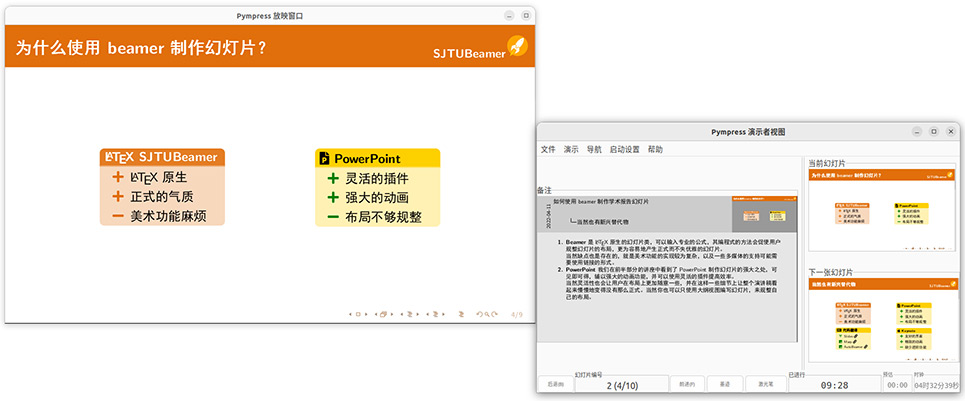
\includegraphics[width=0.7\linewidth]{pympress.jpg}
    \caption{Pympress 阅读器\footnote{需要使用 \cmd{note} 添加笔记,并在导言区添加 \cmd{setbeameroption\{notes on second screen\}} 以启用第二屏功能。} \link{https://github.com/Cimbali/pympress}}
    \note[item]{使用 Pympress 阅读器以最大化 beamer 的交互功能(左侧为放映窗口,右侧为演示者视图),并使用类似于 PowerPoint 演示者视图的界面方便演讲,可便携安装。我也参与了界面的汉化工作。}
    \note[item]{为了使用目前的汉化版本,你需要使用 1.7.2 版本,需要从 PyPi 上手动安装包并且按照指示安装依赖(目前只推荐 \faLinux{} 和 \faApple{} 这么做)。}
    \note[item]{也就是 \texttt{pip install pympress --user} 并安装依赖。之后就是 \texttt{pympress} 启动。}
  \end{figure}

\end{frame}

\section{帧}

\begin{frame}[fragile,label=frame]
  \frametitle{帧}
  \begin{columns}
    \begin{column}{0.5\textwidth}
      \begin{codeblock}{帧}
\documentclass{ctexbeamer}
\begin{document}
|\highlightline<1>|\begin{frame}
|\highlightline<2>|  \frametitle{||beamer 介绍}
|\highlightline<2>|  \framesubtitle{||发起人}
|\highlightline<3>|  beamer 由|| Till Tantau 发起。
|\highlightline<1>|\end{frame}
\end{document}
      \end{codeblock}
    \end{column}
    \begin{column}{0.5\textwidth}
      
      \only<1>{
        \pkg{beamer} 的自然切割单位为 \env{frame}(帧),一帧可以派生出很多张幻灯片(slide)。
      }

      \only<2>{
        \cmd{frametitle} 用于指定该帧的标题,\cmd{framesubtitle} 还可以用来指定该帧的子标题。
      }

      \only<3>{
        \begin{center}
          \includebeamerlarge{frame}
        \end{center}
      }
    \end{column}
  \end{columns}
\end{frame}

\section{渐进切换}

\begin{frame}[fragile]
  \frametitle{占位覆盖}
  
  \begin{columns}
    \begin{column}{0.5\textwidth}
      \begin{codeblock}{暂停式}
\documentclass{ctexbeamer}
\begin{document}
\begin{frame}
|\highlightline<2-4>|    第一段
|\highlightline<1>|  \pause
|\highlightline<3-4>|
|\highlightline<3-4>|    第二段
|\highlightline<1>|  \pause
|\highlightline<4>|        
|\highlightline<4>|    第三段
||\end{frame}
\end{document}
      \end{codeblock}
    \end{column}
    \begin{column}{0.5\textwidth}

      \only<1>{
        \cmd{pause} 用来渐进地展示每一部分的内容,未展示的内容会有占位。
      }

      \only<2-4>{
        \makebox[1cm][l]{\includebeamerlarge[1]{pause}}
      }
      \only<3-4>{
        \makebox[1cm][l]{\includebeamerlarge[2]{pause}}
      }
      \only<4>{
        \makebox[1cm][l]{\includebeamerlarge[3]{pause}}
      }
    \end{column}
  \end{columns}
  
\end{frame}

\begin{frame}[fragile]
  \frametitle{替代覆盖}

  \begin{columns}
    \begin{column}{0.5\textwidth}
      \begin{codeblock}{替代覆盖}
||\documentclass{ctexbeamer}
||\begin{document}
  \begin{frame}
|\highlightline<3->|    \only<2->{||第二}
|\highlightline<2>|    \only<1>{||第一}
|\highlightline<2,4>|    \only<1,3>{||第三}
||  \end{frame}
||\end{document}
      \end{codeblock}
    \end{column}
    \begin{column}{0.5\textwidth}

      \only<1>{

      \cmd{only} 需要通过\alert{修饰符}来指定内容排印的子幻灯片编号,没有显示的内容将不会占位。由于内容没有被实际排印出来,可能会在不同的子幻灯片间产生版面抖动问题。

      \begin{table}
        \centering
        \footnotesize
        \begin{tabular}{>{\color{structure}}cl}
          \texttt{<x>} & 
            \begin{tabular}[t]{l}  
              显示在第 \texttt{x} 子页
            \end{tabular} \\
          \texttt{<x,y>} & 
            \begin{tabular}[t]{l}
              显示在第 \texttt{x} 和第 \texttt{y} 子页上\\
              \scriptsize (每一项也可以是一个范围)
            \end{tabular} \\
          \texttt{<x-y>} & 
            \begin{tabular}[t]{l}
              显示在第 \texttt{x} 到第 \texttt{y} 子页上 \\
              \scriptsize (如果 \texttt{y} 被省略,默认到最后一个子页)
            \end{tabular}
            \\
        \end{tabular}
      \end{table}
      }

      \only<2-4>{
        \begin{center}
          \begin{tikzpicture}
            \node at (0,0) {\includebeamerlarge[1]{only}};
            \only<3->{\node at (0,-2) {\includebeamerlarge[2]{only}};}
            \only<4>{\node at (0,-4) {\includebeamerlarge[3]{only}};}
          \end{tikzpicture}
        \end{center}
      }

      \only<5>{
        与 \cmd{only} 类似的还有 \cmd{alt}、\cmd{temporal}。

        \begin{table}
          \centering
          \footnotesize
          \begin{tabular}{>{\ttfamily}lccc}
             & \scriptsize 1 & \scriptsize 2 & \scriptsize 3 \\
             \midrule
            \cmd{only}<2>\{二\} & & 二 & \\
            \cmd{alt}<2>\{二\}\{一\} & 一 & 二 & 一 \\
            \cmd{temporal}<2>\{一\}\{二\}\{三\} & 一 & 二 & 三 \\
          \end{tabular}
        \end{table}
      }

    \end{column}
  \end{columns}

\end{frame}


\begin{frame}[fragile]
  \frametitle{渐进切换}

  \begin{columns}
    \begin{column}{0.5\textwidth}
      \begin{codeblock}{占位覆盖}
\documentclass{ctexbeamer}
\begin{document}
||  \begin{frame}
|\highlightline<3->|    \onslide<2->{||第二}
|\highlightline<2>|    \onslide<1>{||第一}
|\highlightline<2,4>|    \onslide<1,3>{||第三}
||  \end{frame}
\end{document}
      \end{codeblock}
    \end{column}
    \begin{column}{0.5\textwidth}
      
      \only<1>{
        \cmd{onslide} 可以通过修饰符来指定显示的子幻灯片页码,\cmd{pause} 与此类似但不能指定子页码。
      }

      \only<2-4>{
        \begin{center}
          \begin{tikzpicture}
            \node at (0,0) {\includebeamerlarge[1]{onslide}};
            \only<3->{\node at (0,-2) {\includebeamerlarge[2]{onslide}};}
            \only<4>{\node at (0,-4) {\includebeamerlarge[3]{onslide}};}
          \end{tikzpicture}
        \end{center}
      }

    \end{column}
  \end{columns}
\end{frame}

\begin{frame}
  \frametitle{渐进切换}
  实际上 \cmd{onslide} 是覆盖命令的基础命令,其变种可以等同其他覆盖命令 \link{https://github.com/CTeX-org/beamer-code-cn}。

  \begin{table}
    \centering
    \begin{tabular}{>{\ttfamily}lc>{\ttfamily}l}
      \cmd{pause} & $\Rightarrow$ & \cmd{onslide}<c-> \\
      \cmd{only}<x> & $=$ & \cmd{onslide}*<x> \\
      \cmd{uncover}<x> & $=$ & \cmd{onslide}<x> \\
      \cmd{visible}<x> & $=$ & \cmd{onslide}+<x>\footnote{\cmd{onslide+} 和 \cmd{onslide} 的区别在于前者即使在全局使用透明覆盖模式时 \cmd{setbeamercovered\{transparent\}} 透明度也是无效的(只能全显示或不显示)。} \\
    \end{tabular}
  \end{table}

  渐进切换是 \pkg{beamer} 非常强大的编程模型,合理使用可以减少重复代码的编写。但也希望它的文本参数不要太过复杂,否则可能无法解析。\textsl{Keep It Simple, Stupid.}
\end{frame}

\begin{frame}[fragile]
  \frametitle{列表覆盖}
  \begin{columns}
    \begin{column}{0.5\textwidth}
      \begin{codeblock}{列表覆盖}
\documentclass{ctexbeamer}
\begin{document}
  \begin{frame}
|\highlightline<1>|    \begin{itemize}[<+->]
|\highlightline<2-4>|      \item 第一点
|\highlightline<3-4>|      \item 第二点
|\highlightline<4>|      \item 第三点
    \end{itemize}
||  \end{frame}
\end{document}
      \end{codeblock}
    \end{column}
    \begin{column}{0.5\textwidth}
      
      \only<1>{
        对列表环境添加 \texttt{<+->} 修饰符可以逐项添加覆盖效果。\texttt{<+-|alert@+>} 还可以高亮当前的覆盖项目。
      }
      \only<2-4>{
        \makebox[1cm][l]{\includebeamerlarge[1]{itemizeoverlay}}
      }
      \only<3-4>{
        \makebox[1cm][l]{\includebeamerlarge[2]{itemizeoverlay}}
      }
      \only<4>{
        \makebox[1cm][l]{\includebeamerlarge[3]{itemizeoverlay}}
      }
    \end{column}
  \end{columns}
\end{frame}

\begin{frame}[fragile]
  \frametitle{其他覆盖}
  \begin{columns}[b]
    \begin{column}{0.5\textwidth}
      一些样式命令可以添加与 \cmd{alt} 行为类似的可选修饰符参数(替换覆盖)。
      \begin{table}
        \footnotesize
        \begin{tabular}{lll}
          \toprule
          \cmd{textbf} & \cmd{textmd} & \cmd{textit} \\
          \cmd{textnormal} & \cmd{textrm} & \cmd{textsc} \\
          \cmd{textsf} & \cmd{textsl} & \cmd{texttt} \\
          \cmd{textup} & \cmd{emph} & \cmd{color} \\
          \cmd{textcolor} & \cmd{alert} & \cmd{structure} \\
          \bottomrule
        \end{tabular}
      \end{table}
      \begin{codeblock}[]{样式覆盖}
\textbf<1>{||第一页加粗}
\alert<2>{||第二页强调}
\textcolor<3>{blue}{||第三页变蓝}
      \end{codeblock}
    \end{column}
    \begin{column}{0.5\textwidth}
      区块和定理环境可以添加与 \cmd{onslide} 行为类似的可选修饰符参数(占位覆盖)。
      \begin{table}
        \footnotesize
        \begin{tabular}{lll}
          \toprule
          \env{block} & \env{alertblock} & \env{exampleblock} \\
          \midrule
          \env{theorem} & \env{corollary} & \env{definition} \\
          \env{definitions} & \env{fact} & \env{example} \\
          \env{examples} & \env{proof} &  \\ 
          \bottomrule
        \end{tabular}
      \end{table}
      \vspace*{0.2cm}
      \begin{codeblock}[]{环境覆盖}
\begin{theorem}<2->[||定理名]
||  第二页之后显示该定理。
\end{theorem}
      \end{codeblock}
    \end{column}
  \end{columns}
\end{frame}

\section{断区接续}

\begin{frame}[fragile]
  \frametitle{分栏}
  \begin{columns}[t]
    \begin{column}{.5\textwidth}
      \pkg{beamer} 提供的标准分栏方法是 \env{columns} 环境,硬分栏方法有助于保持设计。
      
      \begin{codeblock}{}
\documentclass{ctexbeamer}
\begin{document}
  \begin{frame}
|\highlightline<1>|    \begin{columns}[c]
|\highlightline<2>|      \begin{column}{.5\textwidth}
        ||第一栏
|\highlightline<2>|      \end{column}
|\highlightline<2>|      \begin{column}{.5\textwidth}
        ||第二栏
|\highlightline<2>|      \end{column}
|\highlightline<1>|    \end{columns}
||  \end{frame}
\end{document}
      \end{codeblock}
      
    \end{column}
    \begin{column}{.5\textwidth}
      如果你想让过长的内容自动分栏,不妨尝试 \pkg{multicol} 宏包中的 \env{multicols} 环境。
      
      \begin{codeblock}{}
\documentclass{ctexbeamer}
|\highlightline|\usepackage{multicol}
\begin{document}
  \begin{frame}
|\highlightline|    \begin{multicols}{2}
      ||所有内容
|\highlightline|    \end{multicols}
||  \end{frame}
\end{document}
      \end{codeblock}

      \only<1>{
        \begin{alertblock}{}
          \env{columns} 环境可以添加可选参数,用于指定两栏纵向对齐方式(\texttt{b},\texttt{c},\texttt{t},\texttt{T})。\textcolor{structure}{$\blacktriangleleft$}
        \end{alertblock}
      }
      
      \only<2>{
        \begin{alertblock}{}
          \env{column} 环境用于分栏,需要强制参数用于指定栏宽。\textcolor{structure}{$\blacktriangleleft$}
        \end{alertblock}
      }
      
    \end{column}
  \end{columns}
  \note[item]{我个人还是蛮推荐使用 \env{multicols} 的,因为 \env{columns} 带来不便的同时,可能会导致一些宏包无法正常工作(比如 \pkg{parskip})。当然对于本幻灯片而言,更多的应当使用 \env{columns} 因为我需要配合 \env{codeblock} 环境排印代码,需要硬分栏(不希望这一栏的代码跑到另一栏的说明中去)。}
\end{frame}

\begin{frame}[fragile]
  \frametitle{断帧接续}
  \note[item]{标题名称断帧接续,意为断开帧继续,也就是自动将一帧的内容切分为多张幻灯片。}
  \begin{columns}[t]
    \begin{column}{0.5\textwidth}
      对 \env{frame} 环境赋予 \pkg{allowframebreaks} 参数,一张幻灯片内多余的内容就会流入到下一张幻灯片中。
      
      \begin{codeblock}[]{}
\documentclass{ctexbeamer}
\usepackage{zhlipsum}
||\begin{document}
|\highlightline|  \begin{frame}[allowframebreaks]
    \zhlipsum[1-2]
||  \end{frame}
||\end{document}
      \end{codeblock}

      \begin{alertblock}{}
        \pkg{allowframebreaks=0.8} 将指定每一个子页的高度占比不超过 0.8\cmd{textheight}。\textcolor{structure}{$\blacktriangle$}
      \end{alertblock}
      
    \end{column}
    \begin{column}{0.5\textwidth}
      对于数学公式而言,可以对 \env{frame} 环境\textbf{再}赋予 \pkg{allowdisplaybreaks} 参数,就可以对公式按行截断。

      \begin{codeblock}{}
\documentclass{ctexbeamer}
\begin{document}
|\highlightline|    \begin{frame}[allowframebreaks,
|\highlightline|  allowdisplaybreaks]
\begin{align*}
    a =& b  \\
       &+ c \\
    % 长公式...
\end{align*}
||    \end{frame}
||\end{document}
      \end{codeblock}
    \end{column}
  \end{columns}
\end{frame}

\begin{frame}[fragile]
  \frametitle{自动切割}
  \begin{block}{}
    \begin{description}
      \item[\faExclamationTriangle] 慎用断帧接续,会导致渐进切换无法使用!
      \item[\faExclamationTriangle{} \faExclamationTriangle{}] 慎用全局自动切割,滥用将降低可维护性!
    \end{description}
  \end{block}
  \note[item]{这将导致后面的并行程序失效,变成了 \LaTeX{} 串行排版,毕竟鱼和熊掌不可兼得。}
  \note[item]{\LaTeX{} 幻灯片工具人震怒。}
  紧急的时候,可以尝试配合 \cmd{framebreak} 手动分割子页进行全局幻灯片自动切分。
  \begin{columns}
    \begin{column}{0.5\textwidth}
      \begin{codeblock}[]{}
\documentclass{beamer}
|\highlightline|\usepackage{autobeamer}
\begin{document}
    \begin{frame}[allowframebreaks=0.8,fragile]
        % Your full article ...
||    \end{frame}
||\end{document}
      \end{codeblock}
      \begin{alertblock}{}
        更多详见 AutoBeamer 的 \faCodeBranch{} \pkg{pkg} 分支 \link{https://github.com/LogCreative/AutoBeamer/tree/pkg}
      \end{alertblock}
    \end{column}
    \begin{column}{0.5\textwidth}
      \begin{codeblock}[]{autobeamer.sty}
\def\section#1{\par\framebreak
  {\bfseries \color{red} #1}}
\def\chapter#1{\framebreak
  \vspace*{0.3\paperheight}
  \begin{center}
    \Large\color{red} #1 
  \end{center}
  \vspace*{0.3\paperheight}
  \newpage}
      \end{codeblock}
    \end{column}
  \end{columns}
  \note{AutoBeamer 自动切割未来可能是一个较大的程序,要想真的完成自动从论文生成幻灯片,需要将后文的那些机制都结合起来,如果我有时间的话或许会写成 VS Code 插件。再高级点就要加 Machine Learning,提取每一段语义的思想分割并生成标题,这个 idea 或许有商业价值,但我觉得谁想做谁做吧,现在还是处于相对初级的阶段。}
\end{frame}

\section{跳转}

\begin{frame}[fragile,label=jump]
  \frametitle{引用跳转}
  最基本的跳转方式是对 \env{frame} 添加一个标签,之后使用 \cmd{ref} 该标签跳转。
  
  \begin{columns}
    \begin{column}{0.5\textwidth}
      \begin{codeblock}[]{}
\documentclass{ctexbeamer}
\begin{document}
|\highlightline|  \begin{frame}[label=target]
    ||跳转到的帧。
||  \end{frame}
  \begin{frame}
|\highlightline|    ||详见第 \ref{target} 页。
||  \end{frame}
||\end{document}
      \end{codeblock}
    \end{column}
    \begin{column}{0.5\textwidth}
      \begin{center}
        \includebeamerlarge[2]{label}
      \end{center}
    \end{column}
  \end{columns}
\end{frame}

\begin{frame}[fragile]
  \frametitle{按钮跳转}
  还可以采用 \cmd{hyperlink} 外加自带的按钮命令跳转。
  \begin{columns}
    \begin{column}{0.5\textwidth}
      \begin{codeblock}[]{}
\documentclass{ctexbeamer}
\begin{document}
|\highlightline|  \begin{frame}[label=target]
    ||跳转到的帧。
||  \end{frame}
  \begin{frame}
|\highlightline|    \hyperlink{target}{
|\highlightline|  \beamergotobutton{||跳转}}
||  \end{frame}
||\end{document}
      \end{codeblock}
    \end{column}
    \begin{column}{0.5\textwidth}
      \begin{table}
        \centering
        \caption{按钮样式}
        \footnotesize
        \begin{tabular}{ll}
          \cmd{beamerbutton} & \hyperlink{jump}{\beamerbutton{跳转}} \\
          \cmd{beamergotobutton} & \hyperlink{jump}{\beamergotobutton{跳转}} \\
          \cmd{beamerskipbutton} & \hyperlink{jump}{\beamerskipbutton{跳转}} \\
          \cmd{beamerreturnbutton} & \hyperlink{jump}{\beamerreturnbutton{跳转}} \\  
        \end{tabular}
      \end{table}
    \end{column}
  \end{columns}
\end{frame}

\section{建议}

\begin{frame}
  \frametitle{注意事项}
  \begin{itemize}
    \item 建议在制作幻灯片时尽量分点展示,分段会导致段与段之间的分界不够明显。
    \item 尽量不使用代码抄录环境,使用时需要在 \env{frame} 上添加 \pkg{fragile} 选项。
    \item 可以多用图标代替文字,比如使用 \pkg{fontawesome5} 宏包。
    \item 尽可能使用矢量图形,大型图片先压缩再插入,必要时开启 \pkg{draft} 选项。
    \item 避免嵌入动画与视频,转而采用超链接的方式。
    \begin{center}
      \ttfamily
      \cmd{href}\{run:地址\}\{链接标识\}
    \end{center}
  \end{itemize}
\end{frame}

\end{shadedsection}
